\documentclass[spanish,A4,]{article}
\usepackage{sans}
\usepackage{amssymb,amsmath}
\usepackage{ifxetex,ifluatex}
\usepackage{fixltx2e} % provides \textsubscript
\ifnum 0\ifxetex 1\fi\ifluatex 1\fi=0 % if pdftex
  \usepackage[T1]{fontenc}
  \usepackage[utf8]{inputenc}
\else % if luatex or xelatex
  \ifxetex
    \usepackage{mathspec}
    \usepackage{xltxtra,xunicode}
  \else
    \usepackage{fontspec}
  \fi
  \defaultfontfeatures{Mapping=tex-text,Scale=MatchLowercase}
  \newcommand{\euro}{€}
\fi
% use upquote if available, for straight quotes in verbatim environments
\IfFileExists{upquote.sty}{\usepackage{upquote}}{}
% use microtype if available
\IfFileExists{microtype.sty}{\usepackage{microtype}}{}
\usepackage{longtable,booktabs}
\usepackage{graphicx}
\makeatletter
\def\maxwidth{\ifdim\Gin@nat@width>\linewidth\linewidth\else\Gin@nat@width\fi}
\def\maxheight{\ifdim\Gin@nat@height>\textheight\textheight\else\Gin@nat@height\fi}
\makeatother
% Scale images if necessary, so that they will not overflow the page
% margins by default, and it is still possible to overwrite the defaults
% using explicit options in \includegraphics[width, height, ...]{}
\setkeys{Gin}{width=\maxwidth,height=\maxheight,keepaspectratio}
\ifxetex
  \usepackage[setpagesize=false, % page size defined by xetex
              unicode=false, % unicode breaks when used with xetex
              xetex]{hyperref}
\else
  \usepackage[unicode=true]{hyperref}
\fi
\hypersetup{breaklinks=true,
            bookmarks=true,
            pdfauthor={},
            pdftitle={},
            colorlinks=true,
            citecolor=blue,
            urlcolor=blue,
            linkcolor=magenta,
            pdfborder={0 0 0}}
\urlstyle{same}  % don't use monospace font for urls
\setlength{\parindent}{0pt}
\setlength{\parskip}{6pt plus 2pt minus 1pt}
\setlength{\emergencystretch}{3em}  % prevent overfull lines
\setcounter{secnumdepth}{0}
\ifxetex
  \usepackage{polyglossia}
  \setmainlanguage{spanish}
\else
  \usepackage[spanish]{babel}
\fi

\title{Arquitectura de computadoras}

\begin{document}
\maketitle

\section{Arquitectura y Organización de
Computadoras}\label{arquitectura-y-organizaciuxf3n-de-computadoras}

¿Cómo \textbf{definimos} una computadora? ¿Cuándo un dispositivo es una
computadora y cuándo decimos que no lo es? En esta unidad, vemos estos
temas y estudiamos los diferentes componentes que tienen las
computadoras.

\subsection{Componentes de una computadora
simple}\label{componentes-de-una-computadora-simple}

En primer lugar, una \textbf{memoria principal}, que es donde se
almacenan todos los datos y las instrucciones de programa. Todo lo que
puede hacer la computadora, lo hace únicamente con contenidos que estén
en la memoria. Para poder procesar un dato, primero hay que hacerlo
llegar a la memoria principal, no importa de dónde venga. Un conjunto de
datos puede estar en disco, en un pendrive, o ser introducido por el
teclado, pero sólo cuando llega a la memoria principal es que puede ser
procesado por la CPU.

La \textbf{CPU, o Unidad Central de Procesamiento}, es el componente que
realmente lleva a cabo los cómputos. Trabaja leyendo instrucciones y
datos de la memoria; y ejecuta esas instrucciones que operan sobre esos
datos. Vamos a hablar mucho más sobre la CPU en esta unidad.

Los \textbf{dispositivos de Entrada y Salida} son todos aquellos
dispositivos que conectamos a la computadora para hacer que el conjunto
CPU + Memoria se comunique con el ambiente.

\begin{itemize}
\itemsep1pt\parskip0pt\parsep0pt
\item
  Con dispositivos como el teclado, mouse, o tableta digitalizadora,
  podemos introducir datos. Son dispositivos de \textbf{entrada}.
\item
  Con dispositivos como pantalla o impresora, podemos hacer que la
  computadora presente los resultados de los cómputos y los entregue al
  usuario. Son dispositivos de \textbf{salida}.
\item
  Algunos dispositivos son de entrada y salida a la vez, como la tarjeta
  de red.
\end{itemize}

Todos estos componentes, y muchos otros que pueden estar o no presentes,
dependiendo de la \textbf{arquitectura}, o modo de construcción, de la
computadora, están conectados entre sí mediante \textbf{buses} o líneas
de interconexión.

\subsubsection{Memoria}\label{memoria}

La memoria es un componente fundamental de la computadora. Está
implementada con circuitos que pueden estar en uno de dos estados
eléctricos, y por esto los llamamos \textbf{biestables}.

Cada circuito biestable puede almacenar la información correspondiente a
un \textbf{bit}. Los bits están agrupados de a ocho formando los
\textbf{bytes}. Estos circuitos, con las tecnologías de hoy, están super
miniaturizados y contienen muchos millones de posiciones donde se pueden
almacenar temporariamente los datos y las instrucciones de programa.

Para poder utilizar la memoria es imprescindible conocer el número, o
\textbf{dirección}, de la posición de memoria donde está el dato o
instrucción que se necesita acceder. Con esta dirección podemos
\textbf{recuperar}, es decir, \textbf{leer}, el valor que está alojado
en ese byte de la memoria, o escribir sobre ese byte un contenido de
ocho bits.

\subsubsection{CPU}\label{cpu}

La CPU está implementada como un circuito sumamente complejo que
contiene \textbf{registros}. Éstos son lugares de almacenamiento
temporario de datos e instrucciones que se utilizan durante el cómputo.

Si, en un momento dado, sacamos una foto instantánea de una CPU, sus
registros tendrán un cierto conjunto de valores. Ese conjunto de valores
se llama el \textbf{estado} de la CPU. La CPU, mientras opera, va
cambiando de estado, es decir, paso a paso va modificando los valores de
sus registros hasta llegar a un resultado de cada instrucción.

Por atravesar esta sucesión de cambios de estado, se dice que una CPU es
un circuito \textbf{secuencial}. Los cambios de estado son disparados
por un \textbf{reloj}, que es un circuito auxiliar que produce pulsos o
impulsos eléctricos que hacen marchar a la CPU.

La CPU puede interpretar un conjunto determinado de instrucciones. Estas
instrucciones han sido definidas en su arquitectura; y son las únicas
que puede ejecutar. El funcionamiento de la CPU está limitado a estas
instrucciones, que son muy básicas, como sumar dos datos, o leer el dato
que está en una determinada dirección de la memoria.

Sin embargo, cuando escribimos una secuencia de instrucciones en la
memoria, es decir, un \textbf{programa}, podemos hacer que la CPU
desarrolle otras tareas que no estaban previstas en su arquitectura. Por
ejemplo, podemos tener una CPU que no sepa multiplicar o dividir, pero
si cuenta con un programa con las instrucciones adecuadas, puede
ejecutar operaciones de multiplicación o división de datos.

La CPU está constituida por varios circuitos componentes o unidades
funcionales, como la \textbf{Unidad de Control} y la \textbf{Unidad
Lógico-Aritmética}.

\begin{itemize}
\itemsep1pt\parskip0pt\parsep0pt
\item
  La Unidad de Control es la que contiene la lógica necesaria para
  \textbf{leer} cada instrucción del programa que está en memoria,
  \textbf{ejecutarla}, y pasar a la \textbf{siguiente} instrucción. Esta
  lógica se llama el \textbf{ciclo de instrucción} y se repite
  \textbf{continuamente} mientras la CPU está funcionando.
\item
  La Unidad Lógico-Aritmética es la que efectivamente realiza los
  cómputos con los datos.
\end{itemize}

\subsection{Arquitectura de Von
Neumann}\label{arquitectura-de-von-neumann}

\subsubsection{Máquina de programa
almacenado}\label{muxe1quina-de-programa-almacenado}

Por supuesto, además de todos esos componentes que hemos nombrado, hay
muchas otras cosas que físicamente forman parte de la computadora; pero
la descripción de la computadora que hemos hecho hasta el momento dice,
por lo menos en líneas generales, los componentes fundamentales que
tiene cualquier computadora actual. Esta descripción puede resumirse
diciendo que la computadora es una \textbf{máquina de Von Neumann o
máquina de programa almacenado}.

En esta clase de máquinas, existe una memoria; que contiene
instrucciones y datos; que como contenidos de esa memoria, no se
diferencian, salvo por la forma como son utilizados.

Estas máquinas ejecutan las instrucciones almacenadas en memoria
secuencialmente, es decir, procediendo desde las direcciones inferiores
de la memoria hacia las superiores, leyendo y ejecutando cada
instrucción y pasando a la siguiente.

\subsubsection{CPU y Memoria}\label{cpu-y-memoria}

En una \textbf{máquina de Von Neumann}, entonces, aparecen dos
componentes básicos fundamentales que son la CPU y la memoria,

la primera conteniendo una \textbf{Unidad de Control, o UC}, para
realizar el \textbf{ciclo de instrucción},

y una \textbf{Unidad Lógico-Aritmética, o ALU}, para el cómputo.

\subsubsection{Buses}\label{buses}

En la máquina existen diferentes clases de buses para interconectar los
componentes:

\begin{itemize}
\item
  \textbf{buses internos} de la CPU para comunicar la UC y la ALU,
\item
  \textbf{buses de sistema} que relacionan la CPU y la memoria,
\item
  y otros \textbf{buses de Entrada/Salida} para comunicar todo el
  sistema con los dispositivos de entrada o de salida.
\end{itemize}

¿En qué momento se utilizará cada clase de bus?

\begin{itemize}
\itemsep1pt\parskip0pt\parsep0pt
\item
  Cuando la UC disponga que se debe ejecutar una instrucción, tal como
  una suma, enviará los datos de partida, y la instrucción, a la ALU a
  través de un bus interno.
\item
  Si la ALU necesita más datos, los obtendrá de la memoria a través de
  un bus de sistema.
\item
  Si la CPU encuentra instrucciones que ordenan presentar el resultado
  del cómputo al usuario, usará un bus de Entrada/Salida para emitir ese
  resultado por pantalla o por impresora.
\end{itemize}

\subsection{Modelo Computacional Binario
Elemental}\label{modelo-computacional-binario-elemental}

Para comprender desde lo más básico cómo opera la computadora,
recurrimos al \textbf{MCBE o Modelo Computacional Binario Elemental},
que es una máquina teórica. El MCBE es una computadora extremadamente
simple, pero que podría ser implementada físicamente, y funcionaría como
la mayoría de las computadoras actuales. Bueno, con muchas menos
capacidades, claro, pero manteniendo lo esencial de las computadoras de
programa almacenado.

\subsubsection{Esquema del MCBE}\label{esquema-del-mcbe}

\begin{figure}[htbp]
\centering
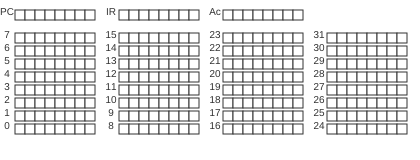
\includegraphics{img/MCBE.png}
\caption{Esquema del MCBE}
\end{figure}

En este esquema del MCBE vemos los tres registros de la CPU: el
\textbf{PC o contador de programa}, el \textbf{IR o registro de
instrucción}, situados en la Unidad de Control, y el
\textbf{Acumulador}, situado en la Unidad Lógico-aritmética. Los tres
son registros de ocho bits.

Además se representa \textbf{la memoria}, compuesta por 32 bytes de ocho
bits. Las direcciones de los bytes van, entonces, \textbf{de 0 a 31}.
Aquí hemos descompuesto la memoria en trozos solamente para poder
representarla completa en el esquema, pero conviene pensar en la memoria
como una única sucesión de bytes, numerados de 0 a 31. Es costumbre, al
representar los diagramas de memoria, ubicar las posiciones con
direcciones menores en la parte inferior del diagrama, y las direcciones
mayores arriba; como si la memoria fuera una escalera con posiciones
numeradas a partir de 0 y ascendiendo.

\textbf{Estado de la máquina}

Cada combinación posible de ceros y unos en los bits de cualquiera de
los registros o posiciones de memoria representa un \textbf{estado} de
la máquina, porque define los valores de la memoria y de los registros
en un momento dado. Es decir, el estado de la máquina en cada momento es
el conjunto de valores de los tres registros y de los 32 bytes de la
memoria.

El estado de la máquina en cada momento define cuál será el estado
siguiente. Ninguna otra cosa interviene en el comportamiento de la
máquina. En particular, la máquina no tiene voluntad ni toma decisiones
propias: solamente cumple el \textbf{ciclo de instrucción}, que la hace
ejecutar las instrucciones del programa que tenga almacenado.

\subsubsection{Memoria del MCBE}\label{memoria-del-mcbe}

Las 32 posiciones de memoria, cada una de 8 bits, son casi todas
iguales, con dos excepciones.

\begin{itemize}
\itemsep1pt\parskip0pt\parsep0pt
\item
  La posición 30 (casi al final de la memoria) está reservada para
  comunicación con dispositivos de entrada. Es sólo de lectura, es
  decir, no se pueden escribir contenidos en esa dirección. Cuando
  leemos esa posición de memoria, la máquina detiene su programa y
  espera que el usuario introduzca un dato. Una vez que el usuario ha
  terminado de escribirlo, el MCBE continúa la operación del programa
  con el dato recién leído.
\item
  La posición 31 es solamente de escritura. Al escribir un dato en la
  dirección 31, hacemos que el MCBE escriba ese valor por pantalla, y
  solamente así podemos saber el resultado de un cómputo.
\end{itemize}

\subsubsection{Registros del MCBE}\label{registros-del-mcbe}

Como hemos dicho, los registros son lugares de almacenamiento temporario
para varios usos. Los registros funcionan en forma parecida a la
memoria, en el sentido de que se pueden leer o escribir datos en ellos,
pero normalmente en una computadora física su velocidad de acceso es
mayor.

Los registros del MCBE tienen diferentes funciones. El registro
\textbf{PC, o contador de programa,} contiene en cada momento la
dirección de la próxima instrucción que se va a ejecutar; es decir,
contiene un número que es la dirección de la posición de memoria donde
está almacenada la instrucción que está por ejecutar el MCBE.

Antes de ejecutar cada instrucción, la CPU va a \textbf{copiarla} en el
registro \textbf{IR, o registro de instrucción}; y mientras está
almacenada allí la instrucción, va a ser decodificada, es decir, la CPU
va a interpretar de qué instrucción se trata, y la va a ejecutar.

El registro \textbf{acumulador}, que pertenece a la ALU, es un registro
que interviene en casi todas las operaciones del MCBE; sobre todo para
las operaciones aritméticas.

\subsubsection{CPU del MCBE}\label{cpu-del-mcbe}

Entonces la CPU del MCBE queda definida como el conjunto de
\textbf{Unidad de Control} con dos registros \textbf{PC e IR}, más
\textbf{Unidad lógico-aritmética} con un registro \textbf{acumulador}.

Esta CPU va a ser muy limitada y solamente va a ejecutar operaciones de
suma y resta en complemento a 2, con ocho bits. No va a ejecutar
\textbf{multiplicaciones}, ni \textbf{divisiones}, ni operaciones en
\textbf{punto flotante}.

\subsubsection{Formato de instrucciones del
MCBE}\label{formato-de-instrucciones-del-mcbe}

\textbf{Código de instrucción} Las instrucciones del MCBE se codifican
en ocho bits y por lo tanto pueden ser almacenadas en un byte de la
memoria, o en el registro IR. Cada instrucción se divide en dos partes:
los tres bits de más a la izquierda se destinan a representar el
\textbf{código de instrucción}.

\textbf{Argumentos u operandos} Los cinco bits restantes representan el
\textbf{argumento u operando} de esa instrucción, es decir, el dato con
el cual tiene que operar esa instrucción.

\textbf{Direcciones y desplazamientos} Por otro lado, los operandos
pueden ser de dos clases: o bien \textbf{direcciones}, o bien
\textbf{desplazamientos}. Si el operando es una dirección, es porque la
CPU necesita conocer la dirección de un dato. Si es un desplazamiento,
ese desplazamiento es \textbf{una cantidad de posiciones} que hay que
trasladarse en la memoria, para encontrar la siguiente instrucción que
hay que procesar.

\begin{itemize}
\itemsep1pt\parskip0pt\parsep0pt
\item
  Cuando el operando es una dirección, los cinco bits del operando
  representan una cantidad sin signo (porque no pueden existir
  direcciones negativas).
\item
  Cuando es un desplazamiento, esos cinco bits son \textbf{con signo}, y
  más precisamente, en complemento a 2; porque el desplazamiento puede
  ser \textbf{negativo}, indicando que hay que \textbf{volver hacia
  atrás, a una cierta dirección de la memoria} a ejecutar una
  instrucción que tal vez ya fue ejecutada.
\end{itemize}

Notemos que al representar las direcciones con cinco bits, sin signo,
tenemos un rango de representación de 0 a 31, justo lo que necesitamos
para alcanzar todas las posiciones de memoria.

Para los desplazamientos, como estamos usando un sistema con signo,
tenemos un rango de -16 a 15. Lo que quiere decir que al trasladarnos de
un lugar a otro de la memoria, vamos a poder hacerlo en saltos de a lo
sumo 16 bytes hacia atrás o 15 bytes hacia adelante.

\subsubsection{Conjunto de instrucciones del
MCBE}\label{conjunto-de-instrucciones-del-mcbe}

Las instrucciones del MCBE se dividen en cuatro grupos.

\begin{itemize}
\itemsep1pt\parskip0pt\parsep0pt
\item
  Las instrucciones de transferencia de datos son las que leen o
  escriben datos en la memoria.\\
\item
  Las aritméticas son las que operan entre esos datos de la memoria y el
  valor presente en el registro acumulador.\\
\item
  Las de salto o transferencia de control, las que desvían, derivan o
  trasladan la ejecución a otra posición de memoria.\\
\item
  Y las de control, completan el funcionamiento de la máquina, por
  ejemplo controlando cuándo va a detenerse el programa.
\end{itemize}

Notemos que, como tenemos un campo de \textbf{tres bits} para definir el
código de instrucción, no vamos a poder tener más que \textbf{ocho
instrucciones}. Precisamente hay dos instrucciones en cada grupo de
estos cuatro que hemos definido.

\textbf{Instrucciones de transferencia de datos}

Las instrucciones de transferencia de datos son dos. El código 010 copia
un byte de la memoria hacia el acumulador. Para esto se necesita la
\textbf{dirección} de ese byte, y esa dirección es precisamente el
argumento u operando de la instrucción, y por lo tanto esa dirección
está codificada en los cinco bits de operando de la instrucción.

El código 011 es la operación inversa, es decir, copia el contenido del
registro acumulador en una posición de memoria. La dirección de esa
posición está, también, determinada por los cinco bits de operando.

En cualquiera de los dos casos, luego de ejecutarse la instrucción, el
valor del PC queda valiendo 1 más de lo que valía antes, es decir, se
incrementa en 1. Esto permite que el ciclo de instrucción pase a la
instrucción siguiente.

El efecto sobre el estado de la máquina es exactamente lo que se
describe aquí: cambia el valor del acumulador, en el caso de la
instrucción 010, o el valor de una posición de memoria, en el caso del
código 011, y el valor del PC se incrementa en 1. No ocurre ningún otro
cambio en el estado de la máquina, ni en los registros ni en la memoria.

\textbf{Instrucciones aritméticas}

Las instrucciones aritméticas también son dos. Si el código es 100, la
CPU va a buscar el valor contenido en la dirección dada por el operando,
y lo suma al acumulador. Es decir, se suman el valor que tuviera
anteriormente el acumulador, con el valor que proviene de esa posición
de memoria. El resultado queda en el acumulador. El valor de la posición
de memoria no varía.

Si el código es 101, la operación es una resta, que como sabemos
consiste en complementar a 2 el operando y luego sumar. El resultado,
igual que en la instrucción de suma, queda en el acumulador, y la
posición de memoria queda sin cambios. Como en las instrucciones de
transferencia de datos, el registro PC se incrementa en 1. Decimos que
el PC \textbf{queda apuntando} a la siguiente instrucción.

\textbf{Instrucciones de salto}

Las dos instrucciones \textbf{de salto, o de transferencia de control},
tienen un efecto diferente. Funcionan modificando exclusivamente el
valor del registro PC. En ambos casos, el operando es un valor con signo
a cinco bits. En el caso del código 110, ese valor se suma
algebraicamente al valor que tuviera hasta el momento el registro PC.
Con lo cual el PC queda apuntando a alguna posición de memoria por
delante o por detrás de donde estaba antes. Así, el ciclo de instrucción
siguiente va a leer la instrucción ubicada en esa nueva dirección que
ahora está contenida en el PC.

El código 110 es una instrucción de salto \textbf{incondicional}, es
decir, \textbf{siempre} provoca un \textbf{salto} en la ejecución. En el
caso del código 111, el salto es \textbf{condicional, y depende del
valor del registro acumulador}. Si el acumulador \textbf{tiene un valor
0}, se produce el salto, sumando el valor del desplazamiento al registro
PC. Pero si el acumulador no vale cero, simplemente se incrementa el PC
en 1 como en el resto de las instrucciones; y el control sigue
secuencialmente como es normal.

\textbf{Otras instrucciones}

Hasta el momento no hemos explicado cómo se detiene la máquina. El ciclo
de instrucción continuamente va a ejecutar la instrucción siguiente, sin
parar nunca. Para terminar la ejecución usamos la instrucción 001. El
programa se detiene, y el estado final de la máquina queda con los
valores que recibieron por última vez los registros y la memoria. El
valor del PC no cambia.

La operación 000 no tiene ningún efecto sobre el estado del MCBE, salvo
incrementar el PC. Ningún otro registro ni posición de memoria cambia su
valor.

\subsection{Ciclo de instrucción}\label{ciclo-de-instrucciuxf3n}

Ahora podemos definir con más rigurosidad lo que se entiende por
\textbf{ciclo de instrucción}. El MCBE inicia su operación con todos los
contenidos de la memoria y registros en 0, y se pone a ejecutar
continuamente el ciclo de instrucción. Para esto repite continuamente
las fases siguientes.

\begin{enumerate}
\def\labelenumi{\arabic{enumi}.}
\itemsep1pt\parskip0pt\parsep0pt
\item
  Copia en el registro IR la instrucción cuya dirección está en el PC.
  Como el PC comienza con un valor 0, esto significa copiar la
  instrucción almacenada en la dirección 0 hacia el IR.
\item
  Decodifica la instrucción, lo que significa separar la instrucción en
  sus dos componentes, que son el código de operación, de tres bits, y
  el operando o argumento, de cinco bits.
\item
  Se ejecuta la instrucción, lo que significa que va a haber algún
  efecto sobre el estado de la máquina. Si es una instrucción de
  transferencia de datos, cambiará el registro acumulador o alguna
  posición de memoria; si es una instrucción aritmética, cambiará el
  valor del registro acumulador; si es de transferencia de control,
  cambiará el valor del PC, etc.
\item
  Una vez ejecutada la instrucción, se vuelve a repetir el ciclo,
  leyendo la siguiente instrucción que haya que ejecutar, que será
  aquella cuya dirección esté contenida en el PC.
\end{enumerate}

\subsection{Programación del MCBE}\label{programaciuxf3n-del-mcbe}

¿Cómo es, entonces, un programa para esta máquina teórica? Es una
sucesión de bytes, que representan instrucciones y datos, contenidos en
la memoria a partir de la dirección 0, y donde cada byte va a ser
interpretado como instrucción o como dato según lo diga el programa.
Como el estado inicial de la máquina es \textbf{con todos los valores en
0}, lo único que puede decirse con seguridad es que \textbf{la primera
posición de la memoria contiene una instrucción}. Pero a partir de allí,
el desarrollo de la ejecución va a ser dado por las instrucciones
particulares que contenga el programa.

\begin{longtable}[c]{@{}cc@{}}
\toprule\addlinespace
Dirección & Contenido
\\\addlinespace
\midrule\endhead
00000 & 01000110
\\\addlinespace
00001 & 10000111
\\\addlinespace
00010 & 01101000
\\\addlinespace
00011 & 00100000
\\\addlinespace
00100 &
\\\addlinespace
00101 &
\\\addlinespace
00110 & 00001100
\\\addlinespace
00111 & 00000001
\\\addlinespace
01000 &
\\\addlinespace
\bottomrule
\end{longtable}

\begin{itemize}
\itemsep1pt\parskip0pt\parsep0pt
\item
  En este programa en particular, la primera instrucción es 010 00110,
  que es una instrucción de transferencia de datos de la posición 6 al
  acumulador.
\item
  La segunda instrucción es 100 00111, que es una suma del valor que
  haya en la posición 7 al acumulador.
\item
  La tercera instrucción es 011 01000, que significa transferir el valor
  que haya en el acumulador a la posición 8.
\item
  Y la cuarta instrucción es 001 00000, que es la instrucción de parada,
  con lo cual termina el programa.
\item
  Todas éstas eran las instrucciones del programa. En las posiciones 6 y
  7 de la memoria tenemos datos almacenados en complemento a 2 sobre
  ocho bits. Estos datos son el número 12, en la posición 6, y el número
  1 en la posición 7.
\item
  En las restantes posiciones de memoria hay contenidos nulos, o sea,
  todos los bits en 0, y no los escribimos para no complicar más el
  diagrama.
\end{itemize}

\subsubsection{Traza de ejecución}\label{traza-de-ejecuciuxf3n}

¿Qué es realmente lo que hace este programa, y cuál es el resultado de
ejecutarlo? Para poder saberlo, lo más conveniente es hacer una
\textbf{traza del programa}. Una traza es un diagrama o planilla donde
preparamos \textbf{columnas} con los nombres de los \textbf{registros,
la memoria y la salida}, para poder ir simulando manualmente la
ejecución, e ir anotando qué valores toman esos registros; es decir,
cuáles son los sucesivos estados del MCBE.

Para cada instrucción que se ejecute usaremos un renglón de la planilla.

En la traza solamente escribiremos los elementos del estado \textbf{que
se modifiquen} en cada paso. En la columna de MEMORIA anotaremos cuándo
hay una operación de escritura en memoria, en la columna de SALIDA
anotaremos cuando haya un contenido que se escriba en pantalla, etc.

Este programa en particular presenta la traza que veremos a
continuación.

Queda como ejercicio seguir la traza e interpretar qué está ocurriendo
en cada momento con cada uno de los registros y las posiciones de
memoria.

\begin{longtable}[c]{@{}cc@{}}
\toprule\addlinespace
Dirección & Contenido
\\\addlinespace
\midrule\endhead
00000 & 01000110
\\\addlinespace
00001 & 10000111
\\\addlinespace
00010 & 01101000
\\\addlinespace
00011 & 00100000
\\\addlinespace
00100 &
\\\addlinespace
00101 &
\\\addlinespace
00110 & 00001100
\\\addlinespace
00111 & 00000001
\\\addlinespace
01000 & 00001101
\\\addlinespace
\bottomrule
\end{longtable}

\subsubsection{Ayuda}\label{ayuda}

\begin{itemize}
\itemsep1pt\parskip0pt\parsep0pt
\item
  000 No operación
\item
  001 Parada
\item
  010 Mem → Ac
\item
  011 Ac → Mem
\item
  100 Sumar al Ac
\item
  101 Restar al Ac
\item
  110 Salto
\item
  111 Salto cond
\end{itemize}

\subsection{Preguntas}\label{preguntas}

\begin{enumerate}
\def\labelenumi{\arabic{enumi}.}
\itemsep1pt\parskip0pt\parsep0pt
\item
  El MCBE, ¿puede encontrar una instrucción que no sea capaz de
  decodificar?
\item
  Supongamos que hemos almacenado en la posición 14 un dato numérico que
  representa la edad de una persona. ¿Qué pasa si en algún momento de la
  ejecución el PC contiene el número 14? ¿Qué pasa si esa persona tiene
  33 años?
\item
  ¿Podría aumentarse la capacidad de memoria del MCBE? ¿Esto requeriría
  algún cambio adicional a la máquina?
\end{enumerate}

Proponemos como ejercicio \textbf{examinar} las siguientes frases,
tomadas de exámenes de la materia, a ver si descubrimos qué está mal en
cada una de ellas.

\begin{enumerate}
\def\labelenumi{\arabic{enumi}.}
\itemsep1pt\parskip0pt\parsep0pt
\item
  El primer paso del ciclo de instrucción es cargar el IR en el PC.
\item
  Lo que hacen las instrucciones de salto es cambiar el efecto de las
  instrucciones en los registros del MCBE.
\item
  Las instrucciones de salto sirven como desplazamiento de instrucciones
  y cambian el orden de los registros.
\item
  La instrucción de salto incondicional es un desplazamiento sin signo,
  la de salto condicional es un desplazamiento con signo.
\item
  Las instrucciones de salto copian el contenido de la dirección en el
  acumulador.
\end{enumerate}

\end{document}
